% ══════════════════════════════════════════════════════════════════════════════
% CHAPTER 5 — METHODOLOGY  [restructured, formula-corrected]
% ══════════════════════════════════════════════════════════════════════════════

This chapter details the methods used to measure the tone of central
bank communication and to estimate its association with financial
market outcomes and future rate decisions. The chapter is organised
around the three-pipeline structure illustrated in
\Cref{fig:framework}: a hand-crafted dictionary
(\Cref{sec:meth_dictionary}), a data-driven Random Forest
(\Cref{sec:meth_rf}), and a fine-tuned BERT sentence-level
classifier (\Cref{sec:meth_bert}) run in parallel on the same
cleaned corpus, each producing a continuous score and a discrete
label. \Cref{secmethregressions} specifies the common econometric
framework (market-reaction regressions for RQ1, next-rate prediction
for RQ2, and the comparison tests) into which all three score
streams feed.

Before turning to the technical details, \Cref{fig:framework}
summarises the analysis framework. A hand-crafted Dictionary, a
data-driven Random Forest, and a fine-tuned BERT classifier run
as parallel pipelines on the same cleaned document corpus, each
producing a continuous score and a discrete label. All three score
streams enter a common econometric framework (market-reaction
regressions for RQ1 and next-rate prediction for RQ2) so that the
three methods can be compared directly on identical outcome
variables and identical samples.

% --------------------------------------------------------------------------
% Fig 5.1 — Three-pipeline framework  [redesigned for v31]
% Solid lines = dictionary; dashed = RF; dotted = BERT
% --------------------------------------------------------------------------
\begin{figure}[htbp]
\centering
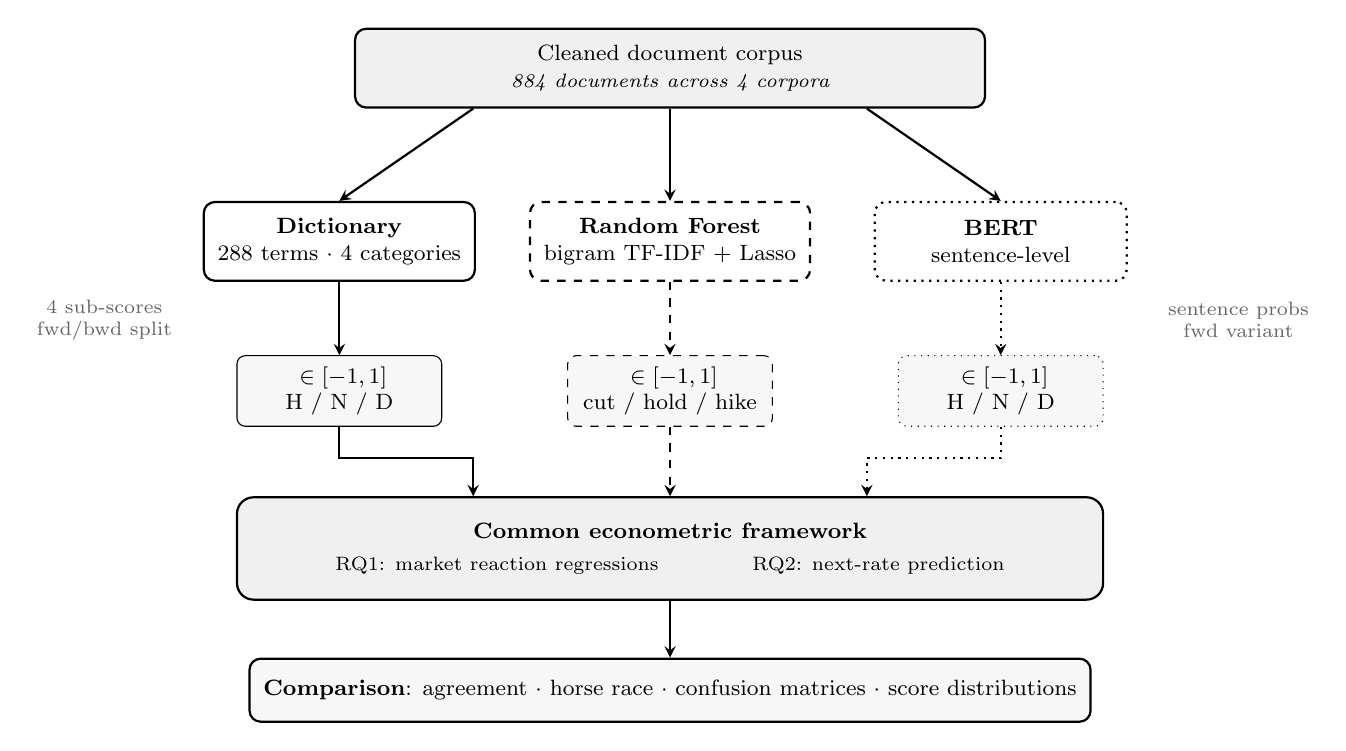
\begin{tikzpicture}[
  every node/.style={font=\footnotesize, align=center},
  inputbox/.style={rectangle, draw=black, thick, minimum height=1.0cm,
                   minimum width=8.0cm, rounded corners=4pt, fill=gray!12,
                   inner sep=5pt},
  dictbox/.style={rectangle, draw=black, thick, minimum height=1.0cm,
                  minimum width=3.2cm, rounded corners=4pt, fill=white,
                  inner sep=5pt},
  rfbox/.style={rectangle, draw=black, thick, minimum height=1.0cm,
                minimum width=3.2cm, rounded corners=4pt, fill=white,
                inner sep=5pt, dashed},
  bertbox/.style={rectangle, draw=black, thick, minimum height=1.0cm,
                  minimum width=3.2cm, rounded corners=4pt, fill=white,
                  inner sep=5pt, dotted},
  scorebox/.style={rectangle, draw=black, minimum height=0.85cm,
                   minimum width=2.6cm, rounded corners=3pt, fill=gray!6,
                   inner sep=4pt},
  regbox/.style={rectangle, draw=black, thick, minimum height=1.3cm,
                 minimum width=11.0cm, rounded corners=6pt, fill=gray!12,
                 inner sep=6pt},
  cmpbox/.style={rectangle, draw=black, thick, minimum height=0.8cm,
                 minimum width=9.0cm, rounded corners=4pt, fill=gray!6,
                 inner sep=5pt},
  arrow/.style={->, thick, >=stealth}
]
  \node[inputbox] (corpus) at (0, 8.5)
    {Cleaned document corpus\\\scriptsize\itshape 884 documents across 4 corpora};
  \node[dictbox] (dict) at (-4.2, 6.3)
    {\textbf{Dictionary}\\288 terms $\cdot$ 4 categories};
  \node[rfbox]   (rf)   at (0, 6.3)
    {\textbf{Random Forest}\\bigram TF-IDF $+$ Lasso};
  \node[bertbox] (bert) at (4.2, 6.3)
    {\textbf{BERT}\\sentence-level};
  \node[scorebox] (ns) at (-4.2, 4.4)
    {\netscore{} $\in [-1,1]$\\H / N / D};
  \node[scorebox, dashed] (rs) at (0, 4.4)
    {\rfscore{} $\in [-1,1]$\\cut / hold / hike};
  \node[scorebox, dotted] (bs) at (4.2, 4.4)
    {\bertscore{} $\in [-1,1]$\\H / N / D};
  \node[font=\scriptsize, text=black!60, anchor=east] at (-6.2, 5.3)
    {4 sub-scores\\fwd/bwd split};
  \node[font=\scriptsize, text=black!60, anchor=west] at (6.2, 5.3)
    {sentence probs\\fwd variant};
  \node[regbox] (regs) at (0, 2.4)
    {\textbf{Common econometric framework}\\[2pt]
     \scriptsize RQ1: market reaction regressions
     \hspace{1.0cm} RQ2: next-rate prediction};
  \node[cmpbox] (cmp) at (0, 0.6)
    {\textbf{Comparison}: agreement $\cdot$ horse race $\cdot$
     confusion matrices $\cdot$ score distributions};
  \draw[arrow] (corpus.south) ++(-2.5,0) -- (dict.north);
  \draw[arrow] (corpus.south) -- (rf.north);
  \draw[arrow] (corpus.south) ++(2.5,0) -- (bert.north);
  \draw[arrow] (dict)   -- (ns);
  \draw[arrow, dashed] (rf) -- (rs);
  \draw[arrow, dotted] (bert) -- (bs);
  \draw[arrow] (ns.south) -- ++(0,-0.4) -| ([xshift=-2.5cm]regs.north);
  \draw[arrow, dashed] (rs.south) -- ++(0,-0.4) -- ([xshift=0cm]regs.north);
  \draw[arrow, dotted] (bs.south) -- ++(0,-0.4) -| ([xshift=2.5cm]regs.north);
  \draw[arrow] (regs)   -- (cmp);
\end{tikzpicture}
\caption[Three-pipeline analysis framework]{Three-pipeline analysis
framework. The same cleaned corpus is processed in parallel by a
hand-crafted Dictionary (\Cref{sec:meth_dictionary}, solid lines),
a data-driven Random Forest (\Cref{sec:meth_rf}, dashed lines),
and a fine-tuned BERT classifier (\Cref{sec:meth_bert}, dotted
lines). Each pipeline produces a continuous score bounded in
$[-1,1]$ and a discrete label. All three streams enter a common
econometric framework (\Cref{sec:meth_regressions}), enabling
direct comparison on identical outcome variables and samples.}
\label{fig:framework}
\end{figure}


% ══════════════════════════════════════════════════════════════════════════════
\section{Dictionary-Based Tone Scoring}
\label{sec:meth_dictionary}
% ══════════════════════════════════════════════════════════════════════════════

\subsection{Design and Term Selection}
\label{sec:meth_dict_selection}

The dictionary approach assumes that the stance of central bank
communication can be approximated from the relative frequency of
hawkish and dovish expressions. In financial text analysis, simple
word-counting methods can capture economically relevant information
when the vocabulary is tailored to the specific domain
\citep{tetlock2007,loughran2011}. This is important because generic
sentiment dictionaries are often poorly suited to financial or
monetary policy text. For example, words such as ``liability'',
``risk'', or ``tightening'' may be classified as negative in a
general sentiment dictionary, but in a central bank setting their
meaning depends on the monetary policy context.

Prior monetary policy dictionaries differ in how they define tone.
\citet{lucca2009} measure the semantic orientation of FOMC
statements by comparing documents to hawkish and dovish benchmark
texts. \citet{picault2017} instead construct an ECB-specific
dictionary that classifies individual terms as hawkish or dovish.
\citet{apel2014} use a similar word-list approach for Riksbank
minutes. This thesis follows the term-level approach and extends it
in three ways: it applies one common dictionary to both FOMC and ECB
communication, focuses on multi-word expressions rather than
isolated words, and separates tone into four economically meaningful
categories: policy action, inflation, employment, and residual risk.
These categories are not meant to be mechanically separate. They are
used to distinguish whether hawkish or dovish language comes from
direct policy language, inflation concerns, labour-market and real
activity assessments, or broader risk communication.

The dictionary was constructed through an iterative,
domain-informed process. Candidate expressions were identified by
reading FOMC statements, ECB introductory statements, and press
conference transcripts, and by reviewing frequently occurring
bigrams and trigrams in the corpus. Terms were retained only if they
satisfied two criteria. First, the expression had to carry a clear
directional meaning in a monetary policy context. Second, it had to
appear often enough to contribute meaningfully to the score. As a
rule, candidate terms were expected to appear at least four times in
the full corpus, while rare expressions with fewer than three
matches were removed. The final dictionary is reported in
\Cref{app:dictionary}.

A central design choice is the exclusion of unigrams. The dictionary
uses only bigrams and trigrams because many monetary policy signals
are phrasal. For example, ``rate hike'' is clearly hawkish, whereas
``rate'' alone is not informative. Similarly, ``above target''
signals inflation pressure, while ``above'' on its own is too vague.
The trigram ``decided raise rates'' captures a direct policy action
more precisely than any single word could. This reduces noise from
isolated words whose meaning depends heavily on context.

Bigrams and trigrams are not perfect, however. They can still miss
negation or subtle context. For example, a phrase such as ``not
expect further tightening'' may contain the hawkish expression
``further tightening'', even though the full sentence is not
hawkish. This limitation motivates the comparison with the
sentence-level RoBERTa/BERT classifier, which uses the full sentence
rather than isolated n-grams.

To match dictionary expressions to the documents, each text is
lowercased, cleaned, tokenised into bigrams and trigrams, and
Porter-stemmed. The same stemming procedure is applied to the
dictionary terms. This ensures that different grammatical forms are
matched consistently: for example, ``raising rates'', ``raised
rates'', and ``raise rates'' are all reduced to the same stemmed
expression. Stop words are removed using the conservative dictionary
stop-word list described in \Cref{sec:data_tokenisation}, while
directional words such as ``above'', ``below'', ``further'', and
``not'' are retained because they can be essential for the meaning
of stance-bearing phrases.

The matching procedure counts bigram and trigram occurrences
separately. Thus, a sentence containing ``decided to raise rates''
may generate both a trigram match for the policy decision and a
bigram match for the rate increase. This additive counting is
intentional: a sentence that contains multiple stance-bearing
expressions provides a stronger signal than a sentence containing
only one. The final document-level score is therefore based on the
balance between hawkish and dovish phrase matches.


\subsection{Semantic Categories and Dual-Mandate Decomposition}
\label{sec:meth_dict_categories}
\label{sec:meth_dual_mandate}

The dictionary terms are organised into four categories: policy
action, inflation, growth and employment, and residual risk. The
purpose of this structure is to make the source of hawkish or
dovish language more transparent. A positive net score may come
from direct rate-hike language, from inflation concerns, from a
strong labour-market assessment, or from broader risk and crisis
vocabulary. Separating these channels allows the empirical analysis
to test whether market reactions are driven by the overall
hawkish--dovish score or by specific parts of the communication.
\Cref{fig:dict_arch} visualises the dictionary structure, and
\Cref{tab:dict_counts} reports the realised term counts.

The first category, \textbf{policy action}, captures direct
references to current or intended policy moves. Hawkish expressions
include ``decided raise,'' ``rate hike,'' ``point increase,''
``further increases,'' and ``raise rates.'' Dovish expressions
include ``decided lower,'' ``point reduction,'' ``rate cut,''
``lower rates,'' and ``policy easing.'' This category is the most
mechanical part of the dictionary because it often describes the
actual policy decision itself. It is therefore useful for detecting
whether a document contains explicit tightening or easing language,
but it also has an important limitation: a rate increase that was
fully expected by markets may still generate hawkish policy-action
language, even if the announcement is not hawkish relative to market
expectations.

The second category, \textbf{inflation assessment}, captures how
the central bank describes price developments. Hawkish inflation
expressions include ``high inflation,'' ``rising inflation,''
``inflation elevated,'' ``price pressures,'' ``cost pressures,''
``second round effects,'' and ``above target.'' Dovish inflation
expressions include ``low inflation,'' ``subdued inflation,''
``falling inflation,'' ``disinflation process,'' ``deflation risk,''
and ``below target.'' This category is central because inflation
language is one of the main ways central banks justify tighter or
looser policy.

The third category, \textbf{growth and employment}, captures
language about real economic activity and labour-market conditions.
Hawkish expressions include ``strong growth,'' ``robust growth,''
``strong demand,'' ``tight labor market,'' ``low unemployment,''
and ``rising wages.'' These phrases are hawkish because they suggest
less need for monetary support and, in some cases, stronger
inflationary pressure. Dovish expressions include ``weak growth,''
``slower growth,'' ``economic weakness,'' ``negative growth,''
``high unemployment,'' ``job losses,'' and ``labor market slack.''
These phrases are dovish because they point to weaker activity or
labour-market slack, which typically supports easier policy. This
category is especially relevant for the FOMC because its mandate
explicitly includes employment, but it is retained for the ECB as
well because ECB communication also discusses growth, demand, and
labour-market conditions when explaining the inflation outlook.

The fourth category, \textbf{residual risk}, contains stance-related
and macro-financial expressions that do not fit cleanly into the
first three categories. Hawkish examples include ``upside risk,''
``strong vigilance,'' ``remain alert,'' ``revised upward,'' and
``stronger than expected.'' Dovish examples include ``downside
risk,'' ``market turmoil,'' ``systemic risk,'' ``zero lower bound,''
``sovereign debt,'' ``financial fragmentation,'' and ``heightened
uncertainty.'' This category is deliberately broad. It captures
risk assessments, crisis language, and financial-stability concerns
that can affect the perceived stance of communication even when the
central bank is not directly discussing rates, inflation, or
employment.

% --------------------------------------------------------------------------
% Fig 5.2 — Dictionary architecture  [redesigned, formula-corrected]
% --------------------------------------------------------------------------
\begin{figure}[htbp]
\centering
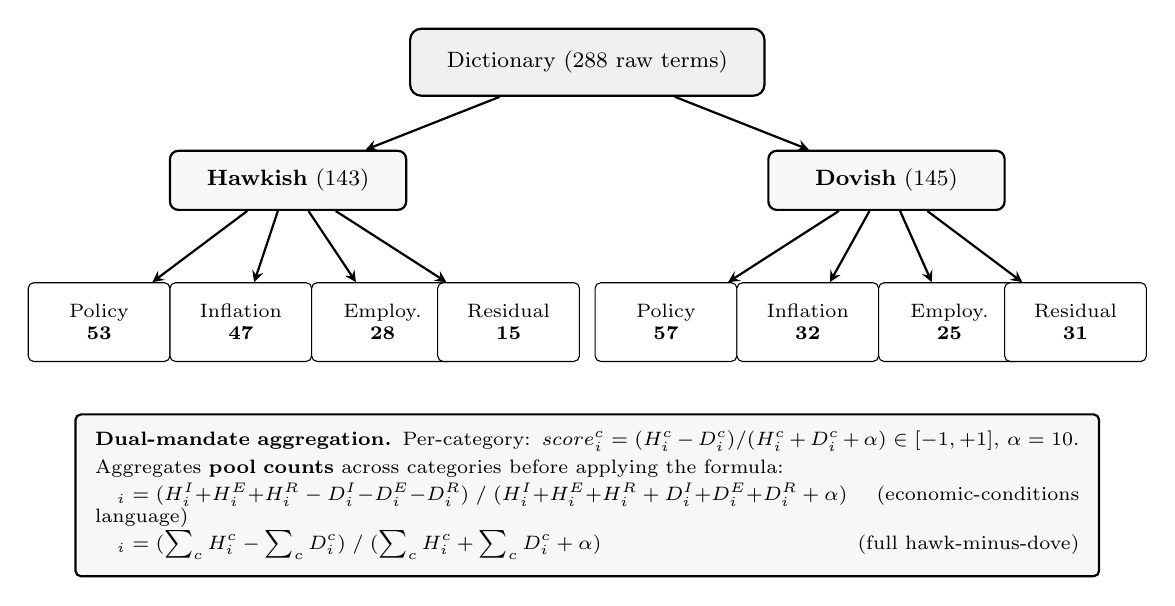
\begin{tikzpicture}[
  every node/.style={font=\footnotesize, align=center},
  rootbox/.style={rectangle, draw=black, thick, minimum height=0.85cm,
                  minimum width=4.5cm, rounded corners=4pt, fill=gray!12},
  dirbox/.style={rectangle, draw=black, thick, minimum height=0.75cm,
                 minimum width=3.0cm, rounded corners=3pt, fill=gray!6},
  catbox/.style={rectangle, draw=black, minimum height=1.0cm,
                 minimum width=1.8cm, fill=white, font=\scriptsize,
                 inner sep=3pt, rounded corners=2pt},
  aggbox/.style={rectangle, draw=black, thick, minimum height=2.0cm,
                 minimum width=13.0cm, fill=gray!6, align=left,
                 text width=12.5cm, font=\scriptsize, inner sep=6pt,
                 rounded corners=2pt},
  arrow/.style={->, thick, >=stealth}
]
  \node[rootbox] (root) at (0, 5.5) {Dictionary (288 raw terms)};
  \node[dirbox] (haw) at (-3.8, 4.0) {\textbf{Hawkish} (143)};
  \node[dirbox] (dov) at ( 3.8, 4.0) {\textbf{Dovish} (145)};
  \node[catbox] (h1) at (-6.2, 2.2) {Policy\\\textbf{53}};
  \node[catbox] (h2) at (-4.4, 2.2) {Inflation\\\textbf{47}};
  \node[catbox] (h3) at (-2.6, 2.2) {Employ.\\\textbf{28}};
  \node[catbox] (h4) at (-1.0, 2.2) {Residual\\\textbf{15}};
  \node[catbox] (d1) at ( 1.0, 2.2) {Policy\\\textbf{57}};
  \node[catbox] (d2) at ( 2.8, 2.2) {Inflation\\\textbf{32}};
  \node[catbox] (d3) at ( 4.6, 2.2) {Employ.\\\textbf{25}};
  \node[catbox] (d4) at ( 6.2, 2.2) {Residual\\\textbf{31}};
  \draw[arrow] (root) -- (haw);
  \draw[arrow] (root) -- (dov);
  \foreach \cat in {h1, h2, h3, h4} \draw[arrow] (haw) -- (\cat);
  \foreach \cat in {d1, d2, d3, d4} \draw[arrow] (dov) -- (\cat);
  \node[aggbox] at (0, 0.0)
    {\textbf{Dual-mandate aggregation.} Per-category:
     $\text{score}^c_i = (H^c_i - D^c_i)/(H^c_i + D^c_i + \alpha)
     \in [-1,+1]$, $\alpha=10$.\\[2pt]
     Aggregates \textbf{pool counts} across categories before
     applying the formula:\\[2pt]
     \quad $\econscore_i =
     (H^I_i{+}H^E_i{+}H^R_i - D^I_i{-}D^E_i{-}D^R_i)\;/\;
     (H^I_i{+}H^E_i{+}H^R_i + D^I_i{+}D^E_i{+}D^R_i + \alpha)$
     \hfill (economic-conditions language)\\
     \quad $\netscore_i =
     (\sum_c H^c_i - \sum_c D^c_i)\;/\;
     (\sum_c H^c_i + \sum_c D^c_i + \alpha)$
     \hfill (full hawk-minus-dove)};
\end{tikzpicture}
\caption[Dictionary architecture]{Dictionary architecture. The 288
raw terms split by direction (143 hawkish, 145 dovish), then
across four semantic categories. The lower panel defines the
dual-mandate aggregation: the four category scores enter
individually (Spec~C), as a policy/economic split (Spec~B), or
pooled into $\netscore{}$ (Spec~A). Aggregate scores pool hawkish
and dovish counts across categories before applying the Laplace-smoothed
$(H{-}D)/(H{+}D{+}\alpha)$ formula, ensuring they remain bounded in
$[-1,+1]$.}
\label{fig:dict_arch}
\end{figure}

\begin{table}[htbp]
\centering
\caption{Dictionary term counts by category, direction, and n-gram type}
\label{tab:dict_counts}
\begin{threeparttable}
\begin{tabular}{lrrrr}
\toprule
Category    & Hawkish & Dovish & Total \\
\midrule
Policy      & 53  & 57 & 110 \\
Inflation   & 47  & 32 & 79  \\
Employment  & 28  & 25 & 53  \\
Residual    & 15  & 31 & 46  \\
\midrule
\textbf{Total} & \textbf{143} & \textbf{145} & \textbf{288} \\
\bottomrule
\end{tabular}
\begin{tablenotes}\footnotesize
  \item[] Counts are raw phrase entries before stemming. After
    Porter stemming and deduplication, 282 unique bigram/trigram
    terms remain. Version~34 of the dictionary; eight entries with
    fewer than three corpus-wide matches were pruned from
    version~33.
\end{tablenotes}
\end{threeparttable}
\end{table}

The final dictionary contains \textbf{282 unique stemmed bigram and
trigram terms}. The hawkish and dovish vocabularies are kept broadly
balanced to avoid mechanically pushing the score in one direction.
The largest category is policy action, followed by inflation, growth
and employment, and residual risk. This reflects the main types of
language through which central banks communicate their policy stance:
direct rate-action language, inflation assessments, real-economy
conditions, and broader risk or crisis-related wording.

The dictionary deliberately excludes unigrams. Single words are often
too ambiguous in monetary policy communication: for example,
``rate,'' ``growth,'' or ``risk'' can appear in hawkish, dovish, or
neutral contexts. Bigrams and trigrams provide more context and are
therefore better suited to identifying directional meaning. A phrase
such as ``rate hike,'' ``above target,'' or ``labor market slack''
contains a much clearer stance signal than any individual word in
isolation.

\Cref{fig:dict_terms_native} illustrates this design choice by
reporting representative high-signal phrases from each category. The
figure is not a substitute for the full dictionary reported in
Appendix~\ref{app:dictionary}; it is intended to show that the
dictionary is built around monetary-policy-specific phrases rather
than generic positive or negative sentiment words.

% --------------------------------------------------------------------------
% Fig 5.3 — Representative dictionary terms [Overleaf-native; no PNG]
% --------------------------------------------------------------------------
\begin{figure}[htbp]
\centering
\small
\setlength{\tabcolsep}{4pt}
\renewcommand{\arraystretch}{1.12}
\begin{tabularx}{\textwidth}{p{1.7cm}XXXX}
\toprule
Direction & Policy action & Inflation & Employment / growth & Residual risk and stance \\
\midrule
Hawkish &
rate hike; point increase; further increases; decided to raise &
high inflation; price pressures; second-round effects; above target &
strong growth; robust growth; rising wages; labour market tightness &
sufficiently restrictive; upside risks; tightening bias; stand ready \\
\addlinespace
Dovish &
rate cut; point reduction; decided to lower; easing measures &
low inflation; subdued inflation; disinflation; below target &
weak growth; slower growth; high unemployment; labour-market slack &
downside risks; accommodation; zero lower bound; fragmentation \\
\bottomrule
\end{tabularx}
\caption[Representative dictionary phrases by semantic category]{Representative
  dictionary phrases by semantic category and direction. The full stemmed
  dictionary is reported in Appendix~\ref{app:dictionary}. The figure is
  generated directly in LaTeX and does not rely on external image files.}
\label{fig:dict_terms_native}
\end{figure}


\subsection{Scoring Formula and Classification}
\label{sec:meth_scoring}
\label{sec:meth_dict_stemming}
\label{sec:meth_dict_ngrams}
\label{sec:meth_threshold}

All dictionary terms and document texts are stemmed using the Porter
stemming algorithm implemented in the \texttt{SnowballC} package
\citep{porter1980}. Stemming reduces related word forms to a common
root, so that, for example, ``raises,'' ``raised,'' and ``raising''
are all matched to the same stem. This avoids the need to list every
grammatical variant of each phrase separately.

Before scoring, the dictionary scorer removes a conservative custom
stop-word list of 44 non-directional function words, including
articles, auxiliary verbs, pronouns, and common connectors. Directional
words such as \emph{above}, \emph{below}, \emph{further}, \emph{more},
\emph{not}, and \emph{still} are deliberately retained because they are
often essential for monetary-policy meaning. For example, ``above
target'' is hawkish, while ``below target'' is dovish; removing these
directional words would destroy the stance signal. The same stop-word
treatment is applied to dictionary phrases and document texts, ensuring
that both sides are matched consistently after preprocessing.

Each document~$i$ is scored separately for the four semantic
categories: policy action, inflation, growth and employment, and
residual risk. For a category $c$, let $H^c_i$ denote the number of
hawkish bigram and trigram matches, and let $D^c_i$ denote the
corresponding number of dovish matches. The category score is then
defined as
\[
    Score^c_i =
    \frac{H^c_i - D^c_i}{H^c_i + D^c_i + \alpha},
    \qquad \alpha = 10.
\]
The constant $\alpha$ stabilises the score for short documents or
documents with few dictionary matches. Without this adjustment, a
single hawkish phrase in a short statement would mechanically produce
a score of one. With the adjustment, isolated matches still affect the
score, but they do not dominate the document-level classification.
This is particularly important for FOMC statements, which are much
\citet{gorodnichenko2023}:
%
\begin{equation}
\label{eq:catscore}
\text{score}^c_i \;=\; \frac{H^c_i - D^c_i}{H^c_i + D^c_i + \alpha},
  \qquad c \in \{P,I,E,R\},
\end{equation}
%
where $\alpha = 10$ is an additive smoothing parameter. The purpose
of this adjustment is to prevent scores from becoming extreme when a
document contains only a small number of directional phrases. Without
the adjustment, a document with one hawkish match and no dovish
matches would receive the maximum score of $+1$, even though the
evidence is weak. With $\alpha=10$, the same document receives
$1/(1+10) \approx 0.09$. The parameter also ensures that the score is
defined when no hawkish or dovish phrase is found.

The score is bounded between $-1$ and $+1$. Positive values indicate
that hawkish phrases dominate, negative values indicate that dovish
phrases dominate, and values close to zero indicate either balanced
language or little directional content. Importantly, the denominator
uses the number of directional dictionary matches rather than total
document length. Normalising by total words would mechanically push
scores toward zero in long press conference transcripts, even when
they contain many stance-relevant phrases. The chosen normalisation
therefore compares hawkish and dovish content conditional on the
amount of stance-bearing language detected in the document.

The four category scores can enter the regression analysis separately
under the dictionary decomposition in
\Cref{sec:meth_dm_decomposition}. Two aggregate scores are also
constructed. These aggregates pool hawkish and dovish counts before
applying the same formula, rather than summing category scores:
%
\begin{align}
\econscore_i &\;=\;
   \frac{(H^I_i + H^E_i + H^R_i) - (D^I_i + D^E_i + D^R_i)}
        {(H^I_i + H^E_i + H^R_i) + (D^I_i + D^E_i + D^R_i) + \alpha},
   \label{eq:econscore}\\[4pt]
\netscore_i &\;=\;
   \frac{\sum_c H^c_i - \sum_c D^c_i}
        {\sum_c H^c_i + \sum_c D^c_i + \alpha}
   \;=\; \frac{H_i - D_i}{H_i + D_i + \alpha},
   \label{eq:netscore}
\end{align}
%
where $H_i = \sum_c H^c_i$ and $D_i = \sum_c D^c_i$ are the total
hawkish and dovish phrase counts across all categories. The
\econscore{} excludes direct policy-action language and focuses on
the central bank's assessment of economic conditions. The
\netscore{} is the broadest dictionary measure and captures the
overall balance of hawkish and dovish language in the document.

For the agreement analysis and label-based comparisons, the
continuous \netscore{} is discretised using a symmetric neutral
band:
%
\begin{equation}
\label{eq:classification}
\text{label}_i =
\begin{cases}
\text{\textsc{hawkish}} & \text{if } \netscore_i > +0.05, \\
\text{\textsc{dovish}}  & \text{if } \netscore_i < -0.05, \\
\text{\textsc{neutral}} & \text{otherwise}.
\end{cases}
\end{equation}
%
The $\pm 0.05$ threshold prevents very small differences between
hawkish and dovish phrase counts from being interpreted as a clear
directional signal. With the additive smoothing parameter
$\alpha=10$, a document must contain a sufficiently large imbalance
between hawkish and dovish matches before it is labelled hawkish or
dovish. For example, 11 hawkish and 10 dovish matches would produce
a score of only \(1/(21+10)=0.032\), and would therefore still be
classified as neutral. By contrast, 11 hawkish and 9 dovish matches
would produce \(2/(20+10)=0.067\), which crosses the hawkish
threshold.

This discretisation is used only for agreement tables and
label-based comparisons. The main regression analysis uses the
continuous \netscore{} directly, so the choice of the neutral-band
threshold does not affect the estimated market-response
coefficients.

\Cref{fig:scoring_example} illustrates the scoring procedure with a
representative text excerpt and shows how matched phrases are
converted into a continuous score and a discrete label.

% --------------------------------------------------------------------------
% Fig 5.3 — Worked example  [redesigned, formula-corrected]
% --------------------------------------------------------------------------
\begin{figure}[htbp]
\centering
\begin{tikzpicture}[
  every node/.style={font=\footnotesize, align=left},
  textbox/.style={rectangle, draw=black, thick, minimum width=13.0cm,
                  inner sep=8pt, rounded corners=3pt, fill=gray!6,
                  text width=12.3cm},
  compbox/.style={rectangle, draw=black, thick, minimum width=13.0cm,
                  inner sep=8pt, rounded corners=3pt, fill=gray!10,
                  text width=12.3cm},
  arrow/.style={->, thick, >=stealth, shorten <=2pt, shorten >=2pt}
]
  % Input text with inline annotations
  \node[textbox] (txt) at (0, 6.0)
    {\textbf{Input} \quad (stylised FOMC-style excerpt)\\[4pt]
     \itshape ``The Committee judges that
     \textbf{ongoing increases}\textsuperscript{\,\textrm{\scriptsize P}}
     in the target range will be appropriate.
     \textbf{Inflation pressures}\textsuperscript{\,\textrm{\scriptsize I}}
     remain elevated, and the labor market continues to be
     \textbf{robust}\textsuperscript{\,\textrm{\scriptsize E}}.
     The Committee is
     \textbf{strongly committed}\textsuperscript{\,\textrm{\scriptsize P}}
     to returning inflation to its 2~percent objective,
     though
     \textbf{downside risks}\textsuperscript{\,\textrm{\scriptsize R}}
     to the outlook persist.''
     \rmfamily\\[4pt]
     Bold $=$ dictionary match.\quad
     Superscripts: P\,$=$\,Policy,
     I\,$=$\,Inflation,
     E\,$=$\,Employment,
     R\,$=$\,Residual.\quad
     Hawkish: 4.\; Dovish: 1.};

  % Computation summary
  \node[compbox] (comp) at (0, 0.8)
    {\textbf{Score computation}
     (Eqs.~\ref{eq:catscore}--\ref{eq:netscore})\\[4pt]
     \begin{tabular}{@{}lllll@{}}
     \toprule
     & Policy & Inflation & Employment & Residual \\
     \midrule
     Hawkish ($H^c_i$) & 2 & 1 & 1 & 0 \\
     Dovish ($D^c_i$)  & 0 & 0 & 0 & 1 \\
     $\text{score}^c_i = \frac{H^c-D^c}{H^c+D^c+\alpha}$
       & $2/12 = 0.17$
       & $1/11 = 0.09$
       & $1/11 = 0.09$
       & $-1/11 = -0.09$ \\
     \bottomrule
     \end{tabular}\\[6pt]
     $\econscore_i = (1{+}1{+}0 - 0{-}0{-}1)/(1{+}1{+}0 + 0{+}0{+}1 + 10)
     = 1/13 = 0.08$.\qquad
     $\netscore_i = (4-1)/(4+1+10) = \mathbf{0.20}$.\qquad
     $> +0.05 \;\Rightarrow\;$ \textbf{\textsc{hawkish}}.};

  \draw[arrow] (txt) -- (comp);
\end{tikzpicture}
\caption[Worked example: text-to-score pipeline]{Worked example
applying the scoring formula to a stylised FOMC-style excerpt.
Matched terms are shown in bold with superscript category labels.
The category scores use $(H^c{-}D^c)/(H^c{+}D^c{+}\alpha)$ per category;
the aggregate $\netscore$ pools all hawkish and dovish counts before
dividing. The $\pm 0.05$ classification threshold assigns a
\textsc{hawkish} label. Note that $\netscore \neq \sum_c
\text{score}^c$: the pooled-count aggregation preserves the $[-1,1]$
bound.}
\label{fig:scoring_example}
\end{figure}


\subsection{Forward/Backward Sentence Decomposition}
\label{sec:meth_fwd_bwd}

To examine whether forward-looking language carries a different
signal from descriptions of current or past conditions, each
document is split into sentences before scoring. A sentence is
classified as \emph{forward-looking} if it contains language that
points to future conditions, future policy decisions, forecasts, or
conditional guidance. All remaining sentences are classified as
\emph{current/backward-looking}.

The classification is based on regular expression patterns for
future-oriented language. These include general future markers such
as ``will,'' ``expected,'' ``future,'' ``outlook,'' and ``prospect'';
forecasting terms such as ``project,'' ``forecast,'' ``foresee,''
and ``trajectory''; policy-intention terms such as ``prepared to,''
``stand ready,'' ``at least until,'' and ``commit to''; and
conditional guidance such as ``data dependent,'' ``meeting by
meeting,'' ``conditional,'' ``contingent,'' and ``if warranted.''
These expressions are used because they identify sentences in which
the central bank discusses what it expects, intends, or may do
rather than simply describing realised developments.

The split is deliberately rule-based and transparent. It does not
claim to perfectly identify all forms of forward guidance, but it
provides a consistent way to separate future-oriented communication
from the rest of the document across both central banks and both
document types. Dictionary scores are then computed separately for
the forward-looking and current/backward-looking parts of each
document, producing \texttt{net\_score\_fwd} and
\texttt{net\_score\_curr}. This allows the empirical analysis to
test whether market reactions are more closely related to language
about the future policy path than to language describing current
economic conditions.

% --------------------------------------------------------------------------
% Fig 5.4 — Forward/backward taxonomy  [redesigned: table format]
% --------------------------------------------------------------------------
\begin{figure}[htbp]
\centering
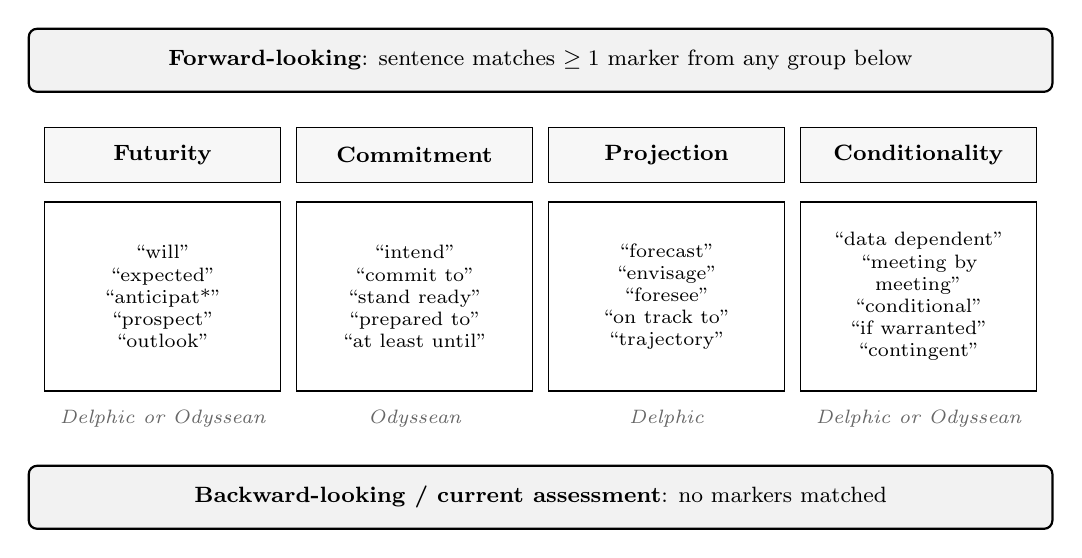
\begin{tikzpicture}[
  every node/.style={font=\footnotesize, align=center}
]
  % Top rule box
  \node[rectangle, draw=black, thick, fill=gray!10,
        minimum width=13.0cm, minimum height=0.8cm,
        rounded corners=3pt, inner sep=4pt]
    at (0, 5.7)
    {\textbf{Forward-looking}: sentence matches $\geq 1$ marker
     from any group below};

  % Column headers
  \node[rectangle, draw=black, fill=gray!6,
        minimum width=3.0cm, minimum height=0.7cm, inner sep=3pt]
    at (-4.8, 4.5) {\textbf{Futurity}};
  \node[rectangle, draw=black, fill=gray!6,
        minimum width=3.0cm, minimum height=0.7cm, inner sep=3pt]
    at (-1.6, 4.5) {\textbf{Commitment}};
  \node[rectangle, draw=black, fill=gray!6,
        minimum width=3.0cm, minimum height=0.7cm, inner sep=3pt]
    at (1.6, 4.5) {\textbf{Projection}};
  \node[rectangle, draw=black, fill=gray!6,
        minimum width=3.0cm, minimum height=0.7cm, inner sep=3pt]
    at (4.8, 4.5) {\textbf{Conditionality}};

  % Keyword columns
  \node[rectangle, draw=black, fill=white,
        minimum width=3.0cm, minimum height=2.4cm,
        inner sep=3pt, font=\scriptsize, text width=2.6cm,
        align=center] at (-4.8, 2.7)
    {``will''\\``expected''\\``anticipat*''\\``prospect''\\``outlook''};
  \node[rectangle, draw=black, fill=white,
        minimum width=3.0cm, minimum height=2.4cm,
        inner sep=3pt, font=\scriptsize, text width=2.6cm,
        align=center] at (-1.6, 2.7)
    {``intend''\\``commit to''\\``stand ready''\\``prepared to''\\``at least until''};
  \node[rectangle, draw=black, fill=white,
        minimum width=3.0cm, minimum height=2.4cm,
        inner sep=3pt, font=\scriptsize, text width=2.6cm,
        align=center] at (1.6, 2.7)
    {``forecast''\\``envisage''\\``foresee''\\``on track to''\\``trajectory''};
  \node[rectangle, draw=black, fill=white,
        minimum width=3.0cm, minimum height=2.4cm,
        inner sep=3pt, font=\scriptsize, text width=2.6cm,
        align=center] at (4.8, 2.7)
    {``data dependent''\\``meeting by\\meeting''\\``conditional''\\``if warranted''\\``contingent''};

  % Campbell et al. mapping row
  \node[font=\scriptsize\itshape, text=black!60] at (-4.8, 1.15)
    {Delphic or Odyssean};
  \node[font=\scriptsize\itshape, text=black!60] at (-1.6, 1.15)
    {Odyssean};
  \node[font=\scriptsize\itshape, text=black!60] at (1.6, 1.15)
    {Delphic};
  \node[font=\scriptsize\itshape, text=black!60] at (4.8, 1.15)
    {Delphic or Odyssean};

  % Bottom else-case box
  \node[rectangle, draw=black, thick, fill=gray!10,
        minimum width=13.0cm, minimum height=0.8cm,
        rounded corners=3pt, inner sep=4pt]
    at (0, 0.15)
    {\textbf{Backward-looking / current assessment}: no markers
     matched};
\end{tikzpicture}
\caption[Forward-looking sentence taxonomy]{Forward-looking sentence
classification. A sentence is classified as forward-looking if it
matches at least one future-oriented marker; otherwise it is treated
as current/backward-looking. The split produces separate dictionary
scores for forward-looking and current/backward-looking text,
$\netscore^{\text{fwd}}_i$ and $\netscore^{\text{curr}}_i$.}
\label{fig:fwbw_taxonomy}
\end{figure}

All sentences that do not match a forward-looking marker are treated
as current/backward-looking language. The two text subsets are then
scored separately using the same dictionary formula as in
Equation~\eqref{eq:netscore}. In other words,
$\netscore^{\text{fwd}}_i$ is the net hawkishness score computed
only from the forward-looking sentences of document~$i$, while
$\netscore^{\text{curr}}_i$ is the same score computed only from the
remaining sentences.

This decomposition is used in the RQ1 market-reaction regressions,
where both scores enter the same specification:
\[
  y_i = \alpha
      + \beta_{\text{fwd}}\netscore^{\text{fwd}}_i
      + \beta_{\text{curr}}\netscore^{\text{curr}}_i
      + \gamma \text{Surprise}_i
      + \varepsilon_i .
\]
For FOMC regressions, the surprise control is MP1 from the USMPD;
for ECB regressions, it is the corresponding short-rate surprise
from the EA-MPD. The outcome \(y_i\) is the event-window market
reaction, such as equity returns, exchange-rate changes, or
two-year yield/OIS reactions.

The purpose is to test whether markets respond more strongly to
language about the future policy path than to language describing
current conditions. If
\(|\beta_{\text{fwd}}| > |\beta_{\text{curr}}|\), this would suggest
that forward-looking communication contains more market-relevant
information than the current-assessment part of the text. The test
therefore links directly to the broader idea that central bank
communication affects markets not only through the current rate
decision, but also through signals about the expected future path of
policy.

% ══════════════════════════════════════════════════════════════════════════════
\section{Random Forest Classifier}
\label{sec:meth_rf}
% ══════════════════════════════════════════════════════════════════════════════

\subsection{Pipeline Design and Feature Engineering}
\label{sec:meth_rf_design}
\label{sec:meth_rf_tfidf}

As a data-driven complement to the hand-crafted dictionary, the RQ1
Random Forest classifier \citep{breiman2001} is trained to predict
the direction of the same-meeting interest rate decision from the
textual content of each document. The target variable is defined as
the sign of the policy-rate change:
%
\begin{equation}
\label{eq:rf_target}
y_i = \text{sign}(\bpschange_i) \in
  \{\text{cut},\; \text{hold},\; \text{hike}\}.
\end{equation}

This is a descriptive classification design. The model learns which
textual patterns are typically associated with realised cuts, holds,
and hikes, and converts these patterns into an alternative
document-level tone measure. The resulting score is therefore not a
pure measure of market-surprise hawkishness. A hike-like document can
still be market-neutral if the rate increase was fully expected, and
a hold can be hawkish or dovish if markets had expected a different
decision. This limitation is important because the true latent object
of interest is not the realised decision itself, but the policy
message relative to expectations.

The empirical design addresses this issue in two ways. First, the RF
classifier is not used as a structural measure of monetary policy
surprises; it is treated as a text-based stance measure and compared
with the dictionary and RoBERTa/BERT scores. Second, the market
reaction regressions include the short-rate surprise control
(MP1 for the FOMC and OIS\_MP1 for the ECB), which captures the
unexpected component of the current rate decision. Conditional on
this control, the coefficient on the RF score is interpreted as the
market response to text associated with policy stance beyond the
immediate rate surprise.

Separate Random Forest models are trained for each of the four
corpora: FOMC statements, FOMC press conferences, ECB statements,
and ECB press conferences. This allows the classifier to learn
institution-specific and document-type-specific language patterns
instead of forcing one common model onto very different types of
central bank communication. Documents with missing rate decisions,
missing text, or fewer than 100 characters are excluded, and all
documents are sorted chronologically before model estimation.

The full pipeline is summarised in \Cref{fig:rf_pipeline}; the
remainder of this section describes the text representation,
feature selection, class-imbalance correction, and construction of
the final RF tone score.

% --------------------------------------------------------------------------
% Fig 5.5 — RF pipeline  [redesigned: B&W with stage-group braces]
% --------------------------------------------------------------------------
\begin{figure}[htbp]
\centering
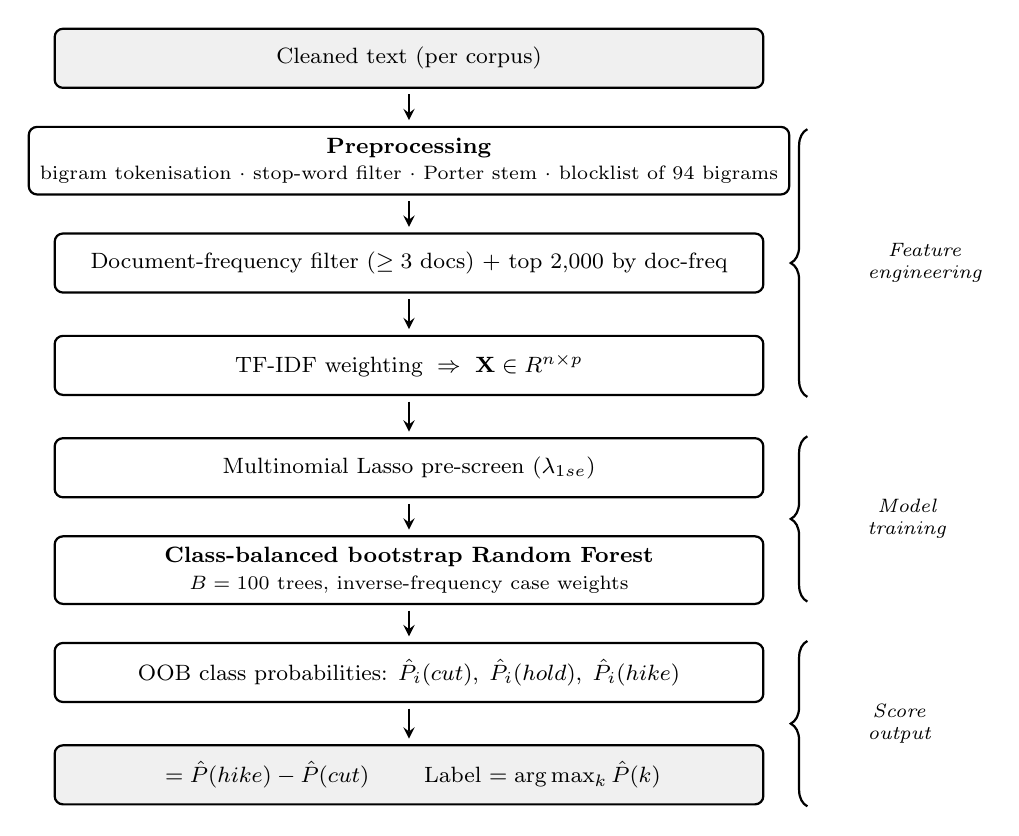
\begin{tikzpicture}[
  every node/.style={font=\footnotesize, align=center},
  pipeblock/.style={rectangle, draw=black, thick, minimum height=0.75cm,
                    minimum width=9.0cm, fill=white, inner sep=4pt,
                    rounded corners=3pt},
  inputblock/.style={pipeblock, fill=gray!12},
  outputblock/.style={pipeblock, fill=gray!12},
  groupbrace/.style={decorate, decoration={brace, amplitude=6pt,
                     mirror, raise=4pt}, thick},
  grouplabel/.style={font=\scriptsize\itshape, anchor=west},
  arrow/.style={->, thick, >=stealth, shorten <=2pt, shorten >=2pt}
]
  \node[inputblock] (in) at (0, 9.5) {Cleaned text (per corpus)};
  \node[pipeblock] (pp) at (0, 8.2)
    {\textbf{Preprocessing}\\\scriptsize bigram tokenisation
     $\cdot$ stop-word filter $\cdot$ Porter stem
     $\cdot$ blocklist of 94 bigrams};
  \node[pipeblock] (df) at (0, 6.9)
    {Document-frequency filter ($\geq 3$ docs)
     $+$ top 2{,}000 by doc-freq};
  \node[pipeblock] (tf) at (0, 5.6)
    {TF-IDF weighting $\;\Rightarrow\;$
     $\mathbf{X}\in\mathbb{R}^{n\times p}$};
  \node[pipeblock] (la) at (0, 4.3)
    {Multinomial Lasso pre-screen ($\lambda_{1\text{se}}$)};
  \node[pipeblock] (bb) at (0, 3.0)
    {\textbf{Class-balanced bootstrap Random Forest}\\
     \scriptsize $B=100$ trees, inverse-frequency case weights};
  \node[pipeblock] (oo) at (0, 1.7)
    {OOB class probabilities:
     $\hat{P}_i(\text{cut}),\;\hat{P}_i(\text{hold}),\;
      \hat{P}_i(\text{hike})$};
  \node[outputblock] (out) at (0, 0.4)
    {\rfscore{} $= \hat{P}(\text{hike}) - \hat{P}(\text{cut})$
     \qquad Label $= \arg\max_k \hat{P}(k)$};
  \draw[arrow] (in) -- (pp);
  \draw[arrow] (pp) -- (df);
  \draw[arrow] (df) -- (tf);
  \draw[arrow] (tf) -- (la);
  \draw[arrow] (la) -- (bb);
  \draw[arrow] (bb) -- (oo);
  \draw[arrow] (oo) -- (out);
  % Stage group braces
  \draw[groupbrace] (5.2, 8.6) -- (5.2, 5.2);
  \node[grouplabel] at (5.7, 6.9) {Feature\\engineering};
  \draw[groupbrace] (5.2, 4.7) -- (5.2, 2.6);
  \node[grouplabel] at (5.7, 3.65) {Model\\training};
  \draw[groupbrace] (5.2, 2.1) -- (5.2, 0.0);
  \node[grouplabel] at (5.7, 1.05) {Score\\output};
\end{tikzpicture}
\caption[Random Forest pipeline]{Random Forest classifier pipeline.
Each corpus is processed independently. Stage groupings are shown
on the right: the feature engineering block reduces the raw bigram
vocabulary through filtering and TF-IDF weighting (Are we really doing TF IDF weighing? I know we build a tf idf matrix but what is tf idf weighting, u mean that we set max 2000 bigrams and then only the top ones go through?; the model
training block applies Lasso pre-screening and fits the
class-balanced forest; the score output block converts OOB
probabilities into a continuous score and discrete label.}
\label{fig:rf_pipeline}
\end{figure}

The feature matrix is constructed through a six-step pipeline:

\begin{enumerate}
  \item \textbf{Tokenisation.} Each document is lowercased and
    tokenised into bigrams. Unigrams are excluded based on
    preliminary experiments showing that bigrams capture
    stance-relevant multi-word expressions that isolated unigrams
    miss, consistent with the importance of phrasal expressions
    documented in Section~\ref{sec:meth_dict_ngrams}.

  \item \textbf{Stop-word filtering.} Bigrams where \emph{either}
    word appears in the stop-word list are removed.

  \item \textbf{Stemming.} Both words in each surviving bigram are
    Porter-stemmed.

  \item \textbf{Blocklist filtering.} 94 stemmed bigrams are removed
    to prevent identity leakage (see below).

  \item \textbf{Document frequency filter.} Bigrams appearing in
    fewer than $\text{MIN\_DOC\_FREQ} = 3$ documents are removed.
    The remaining are ranked by document frequency and the top
    $\text{MAX\_FEATURES} = 2{,}000$ retained.

  \item \textbf{TF-IDF weighting.} Term frequency--inverse document
    frequency weighting produces a document-term matrix
    $\mathbf{X} \in \mathbb{R}^{n \times p}$ where
    $p \leq 2{,}000$.
\end{enumerate}


\subsection{Blocklist, Class Balancing, and Feature Selection}
\label{sec:meth_rf_blocklist}
\label{sec:meth_rf_balanced}
\label{sec:meth_lasso}

An important risk in text classification of institutional documents is
\emph{identity leakage}: the model may learn features that identify the
speaker, institution, or historical period instead of genuine policy
stance. For example, earlier model versions assigned importance to
regional Federal Reserve Bank name pairs, ECB boilerplate, central
banker names, and address fragments. These terms can predict rate
regimes mechanically because certain Chairs or Presidents served during
specific tightening or easing cycles, but they do not themselves contain
hawkish or dovish information.

To reduce this problem, the TF--IDF feature set is filtered using a
blocklist of stemmed bigrams. The blocklist removes institutional
boilerplate, personal names, location references, and other terms that
were judged to identify the document source or period rather than the
policy message. The full blocklist is reported in
\Cref{app:blocklist}. This step forces the classifier to rely more on
substantive language such as inflation pressure, easing, tightening,
labour-market strength, or financial stress.

The classification problem is highly imbalanced because hold decisions
account for the majority of meetings. Without correction, a model could
achieve high headline accuracy simply by predicting ``hold'' too often.
The Random Forest is therefore estimated with class-balanced case
weights. In the code, each observation receives a weight inversely
proportional to the frequency of its class:
%
\begin{equation}
w_i \propto \frac{1}{n_k},
\end{equation}
%
where \(n_k\) is the number of observations in class \(k\). These weights
are passed to \texttt{ranger} through the \texttt{case.weights} argument.
Thus, cut and hike observations receive more weight than hold
observations, preventing the forest from being dominated by the majority
class. Each corpus-specific forest is estimated with \(B=100\) trees.

Because text data generates a very high-dimensional feature space, some
form of feature reduction is necessary before fitting the Random Forest.
Even after restricting the input to bigrams, the number of possible terms
can be large relative to the number of documents. The pipeline therefore
first constructs a TF--IDF matrix from stemmed bigrams and limits the
candidate vocabulary to at most 2{,}000 terms with a minimum document
frequency of three. A multinomial Lasso model is then used as a
pre-selection step. This is implemented through \texttt{cv.glmnet} with
\texttt{family = "multinomial"} and an \(L_1\) penalty:
%
\begin{equation}
\label{eq:lasso}
\hat{\boldsymbol{\beta}}^{\text{Lasso}}
=
\arg\min_{\boldsymbol{\beta}}
\left\{
-\ell(\boldsymbol{\beta}; \mathbf{X}, \mathbf{y})
+
\lambda \sum_{j=1}^{p} |\beta_j|
\right\}.
\end{equation}
%
The Lasso is cross-validated using 10 folds. The preferred penalty is
\(\lambda_{\text{1se}}\), the most parsimonious value within one standard
error of the minimum cross-validation error. If this leaves fewer than
five features, the model switches to \(\lambda_{\min}\). The selected
features are the union of all bigrams with non-zero coefficients across
the cut, hold, and hike classes. The Random Forest is then trained only
on this reduced feature set.

Model performance is evaluated using three measures. First, out-of-bag
(OOB) accuracy uses the internal bootstrap structure of the Random
Forest. Each tree is trained on a bootstrap sample of the data, meaning
that some observations are not used in that tree. These omitted
observations are the out-of-bag observations. The forest can therefore
predict each document using only trees that did not train on that
document, giving an internal estimate of classification performance
without a separate validation set. Second, balanced accuracy averages
recall across the cut, hold, and hike classes, making it more informative
than raw accuracy in an imbalanced setting. Third, chronological holdout
accuracy is computed by training on the first 80\% of observations and
testing on the final 20\%, sorted by date. This provides a simple
time-ordered check of whether the learned text patterns generalise to
later meetings.
%
\begin{equation}
\label{eq:balanced_acc}
\text{Balanced Accuracy} = \frac{1}{K} \sum_{k=1}^{K}
  \frac{\text{TP}_k}{\text{TP}_k + \text{FN}_k},
  \qquad K=3.
\end{equation}


\subsection{Score Construction and Feature Importance}
\label{sec:meth_rf_score}
\label{sec:meth_rf_importance}
\label{sec:meth_model_selection}

The Random Forest produces class probabilities for each document. In
\texttt{ranger}, each tree votes for one of the three classes
\(\{\text{cut},\text{hold},\text{hike}\}\). With
\texttt{probability = TRUE}, these votes are converted into estimated
class probabilities. For a given document, the estimated probability of a
hike is therefore the share of relevant trees that classify the document
as hike-like, and analogously for cuts and holds.

The main RF score is constructed from the out-of-bag class
probabilities:
%
\begin{equation}
\label{eq:rfscore}
\rfscore_i
=
\hat{P}^{\text{OOB}}_i(\text{hike})
-
\hat{P}^{\text{OOB}}_i(\text{cut}).
\end{equation}
%
The score ranges from \(-1\) to \(+1\). Positive values indicate that
the document looks more similar to hike documents than to cut documents;
negative values indicate the opposite. Hold probabilities enter
indirectly: a document with a high hold probability will usually have
both low hike and low cut probabilities, producing an \(\rfscore_i\)
close to zero.

The use of out-of-bag probabilities reduces overfitting. Each tree is
trained on a bootstrap sample of the corpus. Observations not included
in a given tree's bootstrap sample are out-of-bag for that tree. The OOB
probability for document \(i\) is computed only from trees that did not
train on document \(i\). The resulting score is therefore an internal
cross-validated measure of how hike-like or cut-like the document is.
The discrete RF label is assigned as
\[
\text{rf\_label}_i
=
\arg\max_{k \in \{\text{cut},\text{hold},\text{hike}\}}
\hat{P}^{\text{OOB}}_i(k).
\]

Feature importance is measured using Mean Decrease in Gini impurity,
which records how much a bigram improves class separation when it is
used for splits across the forest. Since this importance measure is not
directional, direction is assigned separately by comparing average
TF--IDF values in hike and cut documents:
%
\begin{equation}
\label{eq:direction}
\text{direction}_j
=
\overline{x}_{j|\text{hike}}
-
\overline{x}_{j|\text{cut}}.
\end{equation}
%
A positive value means that bigram \(j\) is more common in hike
documents and is therefore interpreted as hawkish. A negative value means
that the bigram is more common in cut documents and is interpreted as
dovish. The top directional features are ranked by combining predictive
importance with this directional signal. This produces a data-driven
list of stance-bearing bigrams that can be compared with the
hand-crafted dictionary.

\subsection{Forecasting Variants and Expanding Window}
\label{sec:meth_rf_rq2}

The same-meeting Random Forest described above is used for RQ1, where
the goal is to construct an alternative tone measure for the
market-reaction regressions. RQ2 is different. It asks whether language
at meeting \(t\) contains information about future policy decisions or
future market-based rate expectations. For this purpose, the thesis
estimates separate Random Forest regression models in an expanding-window
forecasting design.

Four targets are predicted for each corpus. The variables
\texttt{bps\_next} and \texttt{bps\_next2} are the policy-rate changes
at the next meeting and two meetings ahead. The variables
\texttt{y2\_next} and \texttt{y2\_next2} are the corresponding
one-meeting-ahead and two-meeting-ahead two-year yield or OIS
event-window reactions. The rate-decision forecasts use the current
rate change, \texttt{bps\_curr}, as the inertia benchmark. The yield
forecasts use the current two-year yield or OIS reaction,
\texttt{y2\_curr}, as the corresponding benchmark.

The expanding-window procedure is designed to avoid look-ahead bias.
The first 30 documents form the initial training sample. The model is
then trained on documents \(1,\dots,t-1\) and used to predict the target
for document \(t\). After each prediction, the window expands by one
observation. Thus, the prediction for meeting \(t\) never uses text,
targets, vocabulary, or TF--IDF weights from meeting \(t\) or later.

At each forecast step, the TF--IDF vocabulary and inverse-document
frequency weights are fitted only on the training documents. The test
document is then transformed using this frozen training vocabulary. The
Lasso feature-selection step is also estimated only on the training
sample and is refitted every four meetings; between refits, the most
recent selected feature set is reused. A fresh Random Forest regression
is then trained on the selected bigrams and used to generate the
out-of-sample prediction \(\hat{y}^{\text{xw}}_t\). If the Lasso selects
too few features, the model falls back to the 200 most frequent training
bigrams.

Forecast performance is evaluated using only the sequence of
out-of-sample predictions. The reported \(R^2\) and RMSE therefore
measure genuine expanding-window forecasting performance rather than
in-sample fit. This distinction is important because text models can
look strong in-sample while providing limited predictive value when
forced to forecast future meetings.

% ══════════════════════════════════════════════════════════════════════════════
\section{BERT Sentence-Level Classifier}
\label{sec:meth_bert}
% ══════════════════════════════════════════════════════════════════════════════

\noindent\textit{Terminology note.} Throughout the thesis, the
sentence-level transformer benchmark is labelled \emph{BERT} for
readability in the text, tables, and figures. This label refers to the
BERT-family transformer classifier used in the pipeline. The implemented
model is the zero-shot DeBERTa classifier
\texttt{MoritzLaurer/deberta-v3-base-zeroshot-v2.0}, applied through the
Hugging Face zero-shot classification pipeline with the candidate labels
\emph{hawkish}, \emph{dovish}, and \emph{neutral}. The shortened label
``BERT'' is therefore used as a convenient umbrella term and does not
imply that the model is the FOMC-RoBERTa model of \citet{shah2023}.
:contentReference[oaicite:0]{index=0}

As a third scoring method, the transformer classifier is applied at the
sentence level to every document in the corpus. Each document is first
split into sentences, and each sentence is classified as hawkish,
dovish, or neutral. This sentence-level design is important because it
allows the model to evaluate the full wording of a sentence rather than
isolated bigrams or trigrams. Compared with the dictionary and Random
Forest approaches, the transformer can better handle ambiguity,
qualification, and negation. For example, a bigram-based method may treat
``rate increase'' as mechanically hawkish, whereas a full sentence such
as ``a rate increase is not warranted at this stage'' carries a very
different meaning. The transformer benchmark is therefore included to
test whether contextual sentence classification captures information
missed by phrase-based methods.

The zero-shot classifier returns probabilities for the three candidate
labels. For each sentence \(s\), the pipeline stores
\(\hat{p}_{s,\text{hawk}}\), \(\hat{p}_{s,\text{dove}}\), and
\(\hat{p}_{s,\text{neutral}}\), and assigns the sentence to the label
with the highest probability. The sentence-level directional score is
defined as:
%
\begin{equation}
\label{eq:bert_sentence_score}
\text{bert\_score}_{s}
=
\hat{p}_{s,\text{hawk}}
-
\hat{p}_{s,\text{dove}}.
\end{equation}
%
Positive values indicate hawkish sentence content, negative values
indicate dovish sentence content, and values close to zero indicate
either neutral language or balanced hawkish and dovish probabilities.

Document-level BERT scores are constructed by aggregating the
sentence-level classifications within each document. In the final R
pipeline, the number of hawkish and dovish sentence labels is counted for
each document and transformed into the same smoothed net-score structure
used for the dictionary:
%
\begin{equation}
\label{eq:bert_doc_score}
\bertscore_i
=
\frac{H^{BERT}_i - D^{BERT}_i}
     {H^{BERT}_i + D^{BERT}_i + 10},
\end{equation}
%
where \(H^{BERT}_i\) and \(D^{BERT}_i\) denote the number of sentences in
document \(i\) classified as hawkish and dovish, respectively. Neutral
sentences are not included in the numerator. This makes the BERT score
directly comparable to the dictionary score: both are positive for
hawkish documents, negative for dovish documents, and close to zero for
neutral or balanced documents.

The BERT score is used as an external semantic benchmark rather than as a
manually verified ground-truth label. This distinction matters because
the model is not trained specifically on the thesis corpus and may not
perfectly map central bank language into monetary-policy stance in every
institutional context. Its role is therefore comparative: it tests
whether a contextual sentence-level transformer produces market-relevant
tone measures beyond the hand-crafted dictionary and the Random Forest
bigram classifier.

\subsection{Model and Sentence-Level Classification}

The transformer benchmark used in this thesis is a zero-shot
BERT-family classifier, implemented with
\texttt{MoritzLaurer/deberta-v3-base-zeroshot-v2.0}. For readability,
the thesis refers to this model as \emph{BERT}, although the specific
architecture is DeBERTa rather than the FOMC-RoBERTa model of
\citet{shah2023}. The model is applied through a zero-shot
classification pipeline with three candidate labels: \emph{hawkish},
\emph{dovish}, and \emph{neutral}.

For each sentence, the classifier evaluates how strongly the sentence
matches each of the three candidate labels. It then returns a probability
distribution,
\[
\hat{P}(\text{hawkish}), \quad
\hat{P}(\text{dovish}), \quad
\hat{P}(\text{neutral}),
\]
where the three probabilities sum to one. The predicted sentence label is
assigned by the maximum-probability rule:
\[
\widehat{y}_s
=
\arg\max_{k \in \{\text{hawkish},\text{dovish},\text{neutral}\}}
\hat{P}_{s,k}.
\]
Thus, a sentence is labelled hawkish if the hawkish probability is the
largest of the three, dovish if the dovish probability is largest, and
neutral otherwise.

Each document in the corpus is split into sentences, and every sentence
is classified independently. This sentence-level approach is useful
because the model evaluates the full sentence rather than isolated
bigrams or trigrams. It can therefore reduce some ambiguity inherent in
phrase-based methods. For example, a dictionary may match the phrase
``rate increase'' as hawkish, while a full sentence such as ``a rate
increase is not warranted'' has the opposite implication. The transformer
classifier is included to test whether this contextual information
produces a tone measure that differs from the dictionary and Random
Forest approaches.

The sentence-level predictions are stored alongside the
\texttt{is\_forward} indicator from the forward/backward decomposition
(\Cref{sec:meth_fwd_bwd}). This allows the BERT scores to be aggregated
both over the full document and over forward-looking sentences only.

\subsection{Document-Level Aggregation}

Sentence-level predictions are aggregated to the document level using
the same additive smoothing structure as the dictionary score. Let
$n^H_i$ and $n^D_i$ denote the number of sentences in document~$i$
classified as hawkish and dovish, respectively. Neutral sentences are
not counted in the numerator, because they do not contribute a
directional stance signal. The document-level BERT score is defined as
%
\begin{equation}
\label{eq:bertscore}
\bertscore_i \;=\;
  \frac{n^H_i - n^D_i}{n^H_i + n^D_i + \alpha},
  \qquad \alpha = 10.
\end{equation}
%
The score is bounded between $-1$ and $+1$. Positive values indicate
that hawkish sentences dominate dovish sentences, while negative values
indicate the opposite. The smoothing constant shrinks scores toward
zero when a document contains only a small number of directional
sentences. For example, a document with one hawkish sentence and no
dovish sentence receives a score of $1/(1+10)=0.09$, rather than the
extreme value of $+1$. This makes the score less sensitive to isolated
sentence classifications, especially in short statements.

The discrete BERT label is assigned using the same neutral band as the
dictionary score: documents with $\bertscore_i > 0.05$ are labelled
hawkish, documents with $\bertscore_i < -0.05$ are labelled dovish, and
documents between these thresholds are labelled neutral.

A forward-looking variant, $\bertscore^{\text{fwd}}_i$, is constructed
in two steps. First, the forward/backward sentence split described in
\Cref{sec:meth_fwd_bwd} identifies which sentences contain
forward-looking markers such as ``will,'' ``expected,'' ``outlook,''
``data dependent,'' or ``meeting by meeting.'' Second, the BERT
sentence labels are aggregated only over these forward-looking
sentences:
%
\begin{equation}
\label{eq:bertscore_fwd}
\bertscore^{\text{fwd}}_i \;=\;
  \frac{n^{H,\text{fwd}}_i - n^{D,\text{fwd}}_i}
       {n^{H,\text{fwd}}_i + n^{D,\text{fwd}}_i + \alpha},
  \qquad \alpha = 10.
\end{equation}
%
Thus, BERT itself classifies the stance of each sentence, while the
forward-looking restriction is imposed by the separate sentence-level
rule. The forward-only BERT score therefore measures whether the
sentences that refer to the future are predominantly hawkish or dovish.

\subsection{Expanding-Window BERT Forecasts}
\label{sec:meth_bert_xw}

For RQ2, BERT is also used in a forecasting setting. The sentence
classifier itself is applied once to the full corpus and is not
retrained. What is estimated recursively is only the forecasting
regression that maps the document-level BERT score into the target
variable.

The expanding-window procedure mirrors the Random Forest forecasting
design. After sorting each corpus chronologically, the first
30 documents are used as the initial training sample. For each later
meeting \(t\), the model is estimated only on documents
\(1,\dots,t-1\):
%
\begin{equation}
\label{eq:bert_xw_forecast}
y_i
=
\alpha
+
\beta \bertscore_i
+
\gamma \text{control}_i
+
\varepsilon_i,
\qquad i < t.
\end{equation}
%
The fitted coefficients from this training window are then used to
predict the target for meeting \(t\). The procedure is repeated as the
window expands one meeting at a time. Thus, the prediction for meeting
\(t\) never uses outcome information from meeting \(t\) or from any
future meeting.

The same four targets are used as in the Random Forest forecasting
exercise: \texttt{bps\_next}, \texttt{bps\_next2}, \texttt{y2\_next},
and \texttt{y2\_next2}. Rate-decision targets are controlled for using
\texttt{bps\_curr}, while two-year yield targets are controlled for
using \texttt{y2\_curr}. A forward-looking variant is also estimated
where available by replacing the single score with both
\(\bertscore_i\) and \(\bertscore^{\text{fwd}}_i\). This tests whether
future-oriented BERT tone adds predictive information beyond the full
document score.

%\subsection{Identification Strategy}
\label{sec:meth_identification}

The identifying assumption in the event-study regressions is that, within
the narrow announcement window, the central bank announcement is the
dominant source of asset-price movements. This does not mean that the
textual tone scores are interpreted as direct measures of monetary policy
surprises. The scores measure the observed hawkish--dovish stance of the
communication. A market surprise is a different object: it depends on how
the announcement differs from what market participants expected before
the event.

This distinction is important for interpretation. A realised rate hike is
hawkish in a mechanical policy-decision sense, but it is not necessarily
hawkish from the market's perspective. If markets fully expected a
25-basis-point hike and the central bank delivers exactly that, the rate
decision contains little or no surprise. If markets expected a larger
hike, the same realised hike may even be interpreted as dovish. Conversely,
if markets expected no change, the hike is a hawkish surprise. Therefore,
the sign of the realised rate decision is only an imperfect benchmark for
hawkishness and dovishness.

To account for this issue, the baseline market-reaction regressions
control for the contemporaneous rate surprise. Conceptually, the surprise
component is
%
\begin{equation}
\label{eq:rate_surprise}
S_t =
\Delta i_t -
E_{t^-}\!\left(\Delta i_t \mid \mathcal{I}_{t^-}\right),
\end{equation}
%
where \(\Delta i_t\) is the realised policy-rate change and
\(E_{t^-}(\Delta i_t \mid \mathcal{I}_{t^-})\) is the market expectation
formed before the announcement. For the FOMC, this current-rate surprise
is measured by \(MP1_t\). For the ECB, it is measured by \(OIS\_MP1_t\).

The controlled event-study regressions therefore test whether textual
tone explains announcement-window market reactions after conditioning on
the immediate rate-decision surprise. The coefficient on the text score is
interpreted as a conditional high-frequency association between
communication tone and market reactions, not as a pure structural
communication shock.

This limitation is also relevant for the agreement analysis and the
Random Forest classifier. In those parts of the thesis, the realised
rate-decision sign is used as a practical label for hike, hold, and cut
meetings. This label is useful for constructing a benchmark, but it should
not be interpreted as a perfect measure of market-perceived hawkishness.


\subsection{RQ1: Market-Reaction Specifications}
\label{sec:meth_rq1}
\label{sec:meth_expected_signs}
\label{sec:meth_fwd_reg}
\label{sec:meth_dm_decomposition}
\label{sec:meth_rf_reg}
\label{sec:meth_horserace}
\label{sec:meth_fe}

RQ1 tests whether textual tone is associated with high-frequency market
reactions around central bank announcements. The baseline specifications are:
%
\begin{align}
\text{(Naive):}\quad
Y_i &= \alpha + \beta \netscore_i + \varepsilon_i,
   \label{eq:naive}\\[2pt]
\text{(Controlled):}\quad
Y_i &= \alpha + \beta \netscore_i
    + \gamma \text{MP1}_i + \varepsilon_i.
   \label{eq:controlled}
\end{align}
%
The dependent variable \(Y_i\) is the announcement-window reaction of a
financial market outcome. For FOMC regressions, the current-rate surprise is
measured by \(\text{MP1}_i\). For ECB regressions, \(\text{MP1}_i\) is replaced
by \(\text{OIS\_MP1}_i\). All regressions are estimated separately by corpus and
market outcome.

\paragraph{Expected signs.}
Under the standard monetary policy channel, more hawkish tone should raise
interest-rate expectations. This predicts \(\beta > 0\) for yield outcomes.
For equities, the expected sign is usually negative because higher discount
rates reduce equity valuations. For EUR/USD, the sign depends on the central
bank: FOMC hawkishness should lower EUR/USD through dollar appreciation, while
ECB hawkishness should raise EUR/USD through euro appreciation. For equities,
the sign may be weaker or even positive if hawkish communication is interpreted
as good news about economic strength rather than only as tighter policy.

\paragraph{Forward/backward decomposition.}
To test whether future-oriented language carries a stronger market signal than
current-assessment language, the aggregate score is split into forward-looking
and current/backward-looking components:
%
\begin{equation}
\label{eq:fwd_bwd}
Y_i = \alpha
  + \beta_1 \netscore^{\text{fwd}}_i
  + \beta_2 \netscore^{\text{curr}}_i
  + \gamma \text{MP1}_i
  + \varepsilon_i .
\end{equation}
%
This specification is estimated in the same RQ1 market-reaction regressions as
the baseline model. If \(|\beta_1| > |\beta_2|\), forward-looking tone has a
stronger association with announcement-window market reactions than language
describing current conditions.

\paragraph{Dictionary category decomposition.}
The dictionary is also decomposed into policy-action, inflation, employment,
and residual-risk components. This tests whether the aggregate score masks
different market signals across types of central bank language. Three nested
specifications are estimated:
%
\begin{align}
\text{(Spec~A):}\quad
Y_i &= \alpha + \beta \netscore_i
   + \gamma \text{MP1}_i + \varepsilon_i,
   \label{eq:dm_a}\\[2pt]
\text{(Spec~B):}\quad
Y_i &= \alpha
   + \beta_P \text{score}^P_i
   + \beta_E \econscore_i
   + \gamma \text{MP1}_i + \varepsilon_i,
   \label{eq:dm_b}\\[2pt]
\text{(Spec~C):}\quad
Y_i &= \alpha
   + \beta_P \text{score}^P_i
   + \beta_I \text{score}^I_i
   + \beta_E \text{score}^E_i
   + \beta_R \text{score}^R_i
   + \gamma \text{MP1}_i + \varepsilon_i.
   \label{eq:dm_c}
\end{align}
%
Spec~A is the controlled aggregate-score baseline. Spec~B separates direct
policy-action language from broader economic-condition language. Spec~C further
separates economic conditions into inflation, employment, and residual-risk
language. The main interpretation is whether markets react only to the overall
hawkish--dovish balance or whether specific types of language carry separate
information. Inflation language is expected to matter for both central banks,
while employment language is expected to be more relevant for the FOMC because
employment is part of its dual mandate. For the ECB, employment language may be
less important because its formal objective is centred on price stability.

\paragraph{RF, BERT, and horse-race regressions.}
The RQ1 regressions are repeated with the Random Forest and BERT scores:
%
\begin{align}
Y_i &= \alpha + \beta \rfscore_i
    + \gamma \text{MP1}_i + \varepsilon_i,
   \label{eq:rf_controlled}\\[2pt]
Y_i &= \alpha + \beta \bertscore_i
    + \gamma \text{MP1}_i + \varepsilon_i.
   \label{eq:bert_controlled}
\end{align}
%
The three-way comparison includes all three tone measures in the same
regression:
%
\begin{equation}
\label{eq:horserace}
Y_i = \alpha
  + \beta_1 \rfscore_i
  + \beta_2 \netscore_i
  + \beta_3 \bertscore_i
  + \gamma \text{MP1}_i
  + \varepsilon_i .
\end{equation}
%
This specification tests whether the dictionary, Random Forest, and BERT scores
capture overlapping or complementary information. If one score remains
significant while the others lose explanatory power, that score absorbs the
market-relevant information contained in the others. If several scores remain
significant, they capture different dimensions of communication.

\paragraph{Robustness: chair and era fixed effects.}
The baseline and method-comparison regressions are re-estimated with chair and
era fixed effects. Chair fixed effects absorb persistent differences in
communication style across central bank leaders. Era fixed effects absorb
broad regime differences, such as the pre-GFC period, the ZLB/QE period, and the
post-COVID tightening period.

For each outcome, three specifications are reported: (A) the baseline model
without fixed effects; (B) the same model with chair fixed effects; and (C) the
same model with both chair and era fixed effects. These specifications test
whether the estimated tone coefficient is robust to differences in speaker style
and macroeconomic regime. Fixed-effect regressions are estimated using
\texttt{fixest::feols} with heteroskedasticity-robust standard errors.



\subsection{RQ2: Expanding-Window Prediction of Policy Outcomes and Yield Changes}
\label{sec:meth_rq2}

RQ2 tests whether central bank language contains predictive information about
near-term policy decisions and two-year yield changes. The analysis is designed
as an expanding-window forecasting exercise. For each corpus, four targets are
constructed:
%
\begin{align*}
  \texttt{bps\_next}  &\quad \text{rate decision at meeting } t+1,\\
  \texttt{bps\_next2} &\quad \text{rate decision at meeting } t+2,\\
  \texttt{y2\_next}   &\quad \text{two-year yield change at meeting } t+1,\\
  \texttt{y2\_next2}  &\quad \text{two-year yield change at meeting } t+2.
\end{align*}
%
The rate-decision targets ask whether language at meeting \(t\) helps predict
subsequent policy actions. The yield targets ask whether language also predicts
later changes in market-based rate expectations. The two-meeting horizon is
included because policy communication may affect expectations before the actual
rate adjustment is completed; in other words, guidance at meeting \(t\) may
show up with a lag in the policy decision at \(t+2\).

Two forecasting streams are used. The first is an expanding-window Random Forest
regression. At each meeting \(t\), the TF--IDF vocabulary, Lasso feature
selection, and Random Forest model are estimated using only documents dated
before \(t\). The fitted model is then applied to the document at \(t\) to
generate an out-of-sample prediction. The initial training window contains
30 observations. To reduce computation time, the Lasso feature-selection step is
refitted every four meetings; otherwise, the most recently selected feature set
is reused. If the Lasso selects too few features, the model falls back to the
most frequent training bigrams. This is a computational safeguard and does not
change the interpretation of the forecast.

The second stream is an expanding-window BERT forecast. The sentence-level BERT
score is computed once from the text, but the forecasting regression is estimated
recursively. At each meeting \(t\), the regression
%
\begin{equation}
\label{eq:bert_xw}
  Y_i = \alpha_t + \beta_t \bertscore_i + \gamma_t C_i + \varepsilon_i,
  \qquad i < t,
\end{equation}
%
is estimated on past observations only and then used to predict the target for
meeting \(t\). For rate-decision targets, \(C_i\) is the current meeting's rate
change, \texttt{bps\_curr}. For yield targets, \(C_i\) is the current two-year
yield change, \texttt{y2\_curr}. The same control convention is used when
evaluating the Random Forest forecasts.

Forecast performance is evaluated in two ways. First, direct out-of-sample
\(R^2\) compares the expanding-window forecast with a mean benchmark:
%
\begin{equation}
\label{eq:xw_r2}
  R^2_{\text{xw}} = 1 -
  \frac{\sum_t (Y_t-\widehat{Y}_t)^2}
       {\sum_t (Y_t-\bar{Y})^2}.
\end{equation}
%
A positive value means that the text-based forecast improves on the mean
benchmark; a negative value means that it performs worse. Second, an incremental
forecast regression tests whether the text forecast adds information beyond
simple inertia:
%
\begin{equation}
\label{eq:rq2_incremental}
  Y_t = \alpha + \delta \widehat{Y}^{\text{text}}_t + \theta C_t + \varepsilon_t.
\end{equation}
%
This regression asks whether the text forecast explains variation in future
policy or yield changes after controlling for the current rate or yield movement.
This is useful because policy decisions are highly persistent, so a model must
add information beyond the current policy stance to be economically meaningful.

\subsection{Agreement and Comparison Framework}
\label{sec:meth_agreement}
\label{sec:meth_comparison}

Agreement between a tone label and the realised rate decision is defined as:
%
\begin{equation}
\label{eq:agreement}
\text{Agreement}_i =
\begin{cases}
1 & \text{if label} = \text{\textsc{hawkish}} \text{ and } \bpschange_i > 0, \\
1 & \text{if label} = \text{\textsc{neutral}} \text{ and } \bpschange_i = 0, \\
1 & \text{if label} = \text{\textsc{dovish}}  \text{ and } \bpschange_i < 0, \\
0 & \text{otherwise.}
\end{cases}
\end{equation}
%
This is a realised policy-decision benchmark. It measures whether a text label
matches the actual hike, hold, or cut decision. It does not measure whether the
announcement was surprising to markets. This distinction is important because a
rate hike can be market-neutral if it was fully expected, and it can even be
interpreted as dovish if markets expected a larger hike.

To address this limitation, the thesis also constructs a market-surprise
benchmark based on the sign of the high-frequency rate surprise. For the FOMC,
this benchmark uses \(MP1\); for the ECB, it uses \(OIS\_MP1\). A document is
classified as hawkish if the rate surprise is positive, dovish if it is negative,
and neutral if the surprise is close to zero. The realised-rate benchmark and
the market-surprise benchmark therefore capture different objects: the former
captures the actual policy decision, while the latter captures the unexpected
component of the announcement.

Agreement rates are computed separately for each corpus and for each method:
dictionary, Random Forest, and BERT. The analysis also reports agreement by
tone class, by Chair or President, and by monetary policy era. In addition,
\(3 \times 3\) confusion matrices are constructed for every pair of label
sources: dictionary versus Random Forest, dictionary versus BERT, Random Forest
versus BERT, and each method versus both the rate-decision benchmark and the
market-surprise benchmark.

The three-way method comparison is then evaluated along five dimensions:
agreement with realised rate decisions, agreement with monetary policy
surprises, score distributions, pairwise score correlations, and horse-race
regressions. Together, these tests show whether the Random Forest and BERT add
information beyond the dictionary and whether the additional model complexity is
empirically justified.



% --------------------------------------------------------------------------
% Regression specification reference table
% --------------------------------------------------------------------------
\begin{table}[htbp]
\centering
\caption{Summary of regression specifications}
\label{tab:reg_specs}
\begin{threeparttable}
\footnotesize
\setlength{\tabcolsep}{3.2pt}
\renewcommand{\arraystretch}{1.18}
\begin{tabularx}{\textwidth}{@{}
  >{\raggedright\arraybackslash}p{2.55cm}
  >{\raggedright\arraybackslash}p{3.45cm}
  >{\raggedright\arraybackslash}p{2.45cm}
  >{\raggedright\arraybackslash}X
@{}}
\toprule
Specification & Main text variable(s) & Other controls & Purpose \\
\midrule
\multicolumn{4}{@{}l}{\textit{Panel A: RQ1 market-reaction specifications}} \\
\addlinespace[1pt]
RQ1 naive
  & \netscore{} \newline (Eq.~\ref{eq:naive})
  & None
  & Bivariate baseline linking document tone to announcement-window market reactions. \\
\addlinespace
RQ1 controlled
  & \netscore{} \newline (Eq.~\ref{eq:controlled})
  & MP1 / OIS\_MP1
  & Main dictionary specification; isolates tone after controlling for the target-rate surprise. \\
\addlinespace
Dual-mandate Spec~B
  & $\text{score}^{P}$, \econscore{} \newline (Eq.~\ref{eq:dm_b})
  & MP1 / OIS\_MP1
  & Separates policy-action language from economic-conditions language. \\
\addlinespace
Dual-mandate Spec~C
  & $\text{score}^{P}$, $\text{score}^{I}$, $\text{score}^{E}$, $\text{score}^{R}$ \newline (Eq.~\ref{eq:dm_c})
  & MP1 / OIS\_MP1
  & Tests whether the four dictionary sub-dimensions add explanatory power beyond the aggregate score. \\
\addlinespace
Forward/current split
  & $\netscore^{\text{fwd}}$, $\netscore^{\text{curr}}$ \newline (Eq.~\ref{eq:fwd_bwd})
  & MP1 / OIS\_MP1
  & Separates forward-looking guidance language from current-condition assessment. \\
\addlinespace
RF score
  & \rfscore{} \newline (Eq.~\ref{eq:rf_controlled})
  & MP1 / OIS\_MP1
  & Market-reaction regression using the decision-predictive Random Forest tone score. \\
\addlinespace
BERT score
  & \bertscore{} \newline (Eq.~\ref{eq:bert_controlled})
  & MP1 / OIS\_MP1
  & Market-reaction regression using sentence-level semantic tone. \\
\addlinespace
Horse race
  & \rfscore{}, \netscore{}, \bertscore{} \newline (Eq.~\ref{eq:horserace})
  & MP1 / OIS\_MP1
  & Tests whether the three text measures contain distinct market-relevant information. \\
\midrule
\multicolumn{4}{@{}l}{\textit{Panel B: RQ2 expanding-window forecasting specifications}} \\
\addlinespace[1pt]
RF expanding window
  & $\widehat{Y}^{\text{RF,xw}}$ \newline (Eqs.~\ref{eq:xw_r2}, \ref{eq:rq2_incremental})
  & \texttt{bps\_curr} for rate targets; \texttt{y2\_curr} for yield targets
  & Strict expanding-window Random Forest forecasts for \texttt{bps\_next}, \texttt{bps\_next2}, \texttt{y2\_next}, and \texttt{y2\_next2}. \\
\addlinespace
BERT expanding window
  & $\widehat{Y}^{\text{BERT,xw}}$ \newline (Eqs.~\ref{eq:bert_xw}--\ref{eq:rq2_incremental})
  & \texttt{bps\_curr} for rate targets; \texttt{y2\_curr} for yield targets
  & Expanding-window forecast regression using BERT sentence-level tone scores. \\
\bottomrule
\end{tabularx}
\begin{tablenotes}\footnotesize
  \item[] Estimation: OLS with HC1 robust standard errors for market-reaction
  regressions. All RQ1 specifications are estimated separately by corpus and
  outcome. The thesis model pipeline does not use the older dictionary-only
  ordered-probit robustness specification.
\end{tablenotes}
\end{threeparttable}
\end{table}
